\documentclass{report}
\usepackage{graphicx}
\usepackage{listings}
\usepackage{color}
\usepackage[margin=1.2in]{geometry}
\usepackage{courier}
\usepackage{float}
\usepackage[toc,page]{appendix}
\usepackage{hyperref}
\usepackage{pdfpages}

\definecolor{codegreen}{rgb}{0,0.6,0}
\definecolor{codeblack}{rgb}{0,0,0}
\definecolor{codered}{rgb}{0.867,0,0}
\definecolor{backcolour}{rgb}{ 0.95,0.95,0.95}
\definecolor{codeorange}{rgb}{1,0.447059,0}
\definecolor{codegrey}{rgb}{0.1, 0.1, 0.1}
\definecolor{codeblue}{rgb}{0.29, 0.52, 0.56}
\lstdefinestyle{mystyle}{
    basicstyle=\ttfamily\color{codeblack},
    backgroundcolor=\color{backcolour},   
    commentstyle=\color{codered},
    keywordstyle=\color{codeorange},
    numberstyle=\color{codeblack},
    stringstyle=\color{codegreen},
    breakatwhitespace=false,         
    breaklines=true,                 
    captionpos=b,                    
    keepspaces=true,                 
    numbers=left,                    
    numbersep=10pt,                  
    showspaces=false,                
    showstringspaces=false,
    showtabs=false,                  
    tabsize=2
}
 
\lstset{style=mystyle}

\newcommand{\ul}[1]{\underline{#1}}
\newcommand{\ull}[1]{\underline{\underline{#1}}}
\newcommand{\triangleBrac}[1]{\textless{#1}\textgreater}
\newcommand{\un}{\textunderscore}

\begin{document}
\title{CPS3231  - Computer Graphics - Assignment Report}
\author{Daniel Cauchi}
\date{}
\maketitle

\tableofcontents

\chapter{Introduction}
This is the report for the CPS3231 - Computer Graphics assignment, where a clone of the Arkanoid game was implemented in 3D using WebGL. Object spawning, camera movement, physics, illumination and powerups were implemented and are discussed in chapters 2-6 of this report in that order. Additional features are discussed in chapter 7. A video showcase within a README file is also presented in order to show the game working in order. This README file will also contain any additional instructions.

\chapter{Tasks}
\chapter{Task 1 - Object Spawning}
In this chapter, the scene graph will be discussed and how the objects were displayed on screen. The setup of the game will also be discussed so that subsequent sections will flow more easily.

The following files were downloaded from VLE and used as is without modification:
\begin{itemize}
	\item \textbf{light.js}
	\item \textbf{material.js}
	\item \textbf{model.js}
	\item \textbf{matrix.js}
\end{itemize}

The following scripts were downloaded and modified slightly:

\begin{itemize}
	\item \textbf{textures.js}: Removed previous textures and added new ones (listed below) and put the \textit{convertTextures} function inside it.
	\begin{itemize}
		\item wood: used for the bricks
		\item wood2: used for platform
		\item wood3: used for the walls
		\item iron: used for the balls
		\item gold: used for the powerups
		\item oil: used for the bullets
	\end{itemize}

	\item \textbf{scene.js}: Added a \textit{removeNode} function, which takes a string parameter, traverses the scene graph using a depth-first search and when it finds the node with a child whose name corresponds to the given name, sets that child to null and returns.
\end{itemize}

An important script is \textbf{game.js}. This contains important game parameters and variables which are used throughout the game. It contains parameters about the following (in the order in which they are presented in the code [which contains very useful comments])
\begin{itemize}
	\item Number of lives
	\item Wall positions
	\item Number of bricks (rows and columns - for procedural generation)
	\item Platform parameters
	\item Camera parameters
	\item Ball parameters
	\item Powerup parameters
\end{itemize}

Besides these parameters, \textbf{game.js} also contains the physics objects which are used in the game. An array '\textit{keyDown}' of size 256 is initialised to all \textit{false}. When a key on the keyboard is pressed, the index corresponding to the key turns to true, until it is let go at which point the index turns to false again. This is a way to easily detect whether a key is held down or not. For more specific details on the parameters, the comments describe each parameter and its use.

For events which only happen once when a key is pressed down, the \textit{onKeyDown} method is defined. This method, for example, handles the shooting of bullets. A corresponding method \textit{onKeyUp} is also defined, which releases the ball when spacebar is released after being pressed. These two methods are also the functions where the '\textit{keyDown}' elements are set to true or false accordingly.

The \textbf{modelMaker.js} file contains the given \textit{makeSphere} and \textit{makeQuad} functions. \textit{makeSphere} is used for the balls, powerups, bullets and particles. Alongside these, the functions \textit{makeRectangle} and \textit{makeCuboid} were made, which take the dimensions and positions of said shape and generate the vertices for these shapes. The make cuboid makes 6 quads for the 6 faces and combines them together. This is used for the bricks, platforms and walls.

The file \textbf{objectPool.js} contains a function \textit{ObjectPool} which aids object pooling. A pool is defined by the developer, then the function \textit{getNext} can be used to rotate (iterating where the 'queue' is circular so when it reaches the end, it start from the beginning) trough the objects in the pool. This is done as both an optimisation as well as a simplification step, so that objects do not need to be continuously created and destroyed. These pools are used for the particles, additional balls, bullets and powerups.

Within the \textbf{script.js} file, the rest of the functionality happens. This file contains the \textit{main} function which does the following (in order):
\begin{enumerate}
	\item Defines helper variables for matrices and vectors
	\item Sets up the canvas
	\item Initialises the game variable from \textbf{game.js} and adds its \textit{onKeyUp} and \textit{onKeyDown} methods to the event listeners
	\item Initialise the scene graph
	\item Creates a sphere and cuboid primitive (of unit lengths/radius and position origin)
	\item Sets up geometry for the items (walls, platform, balls, bricks, powerups, bullets and particles)
	\item Creates physics objects for each required item (discussed in the physics section) (Note: while 1 brick can be defined in regards to geometry, then replicated within the scene graph, each single brick would need its own physics item. This is the same for any object for which there are multiple)
	\item Sets up the different lights
	\item Initialise textures from \textbf{textures.js}
	\item Create the separate materials
	\item Assign the materials to the objects
	\item Sets up the scene graph (Discussed below)
	\item Creates the animate function which handles movement (discussed in the physics section)
	\item Calls the animate function
\end{enumerate}

The following is an image of the scene at the start of a game:
\begin{figure}[H]
	\centering
	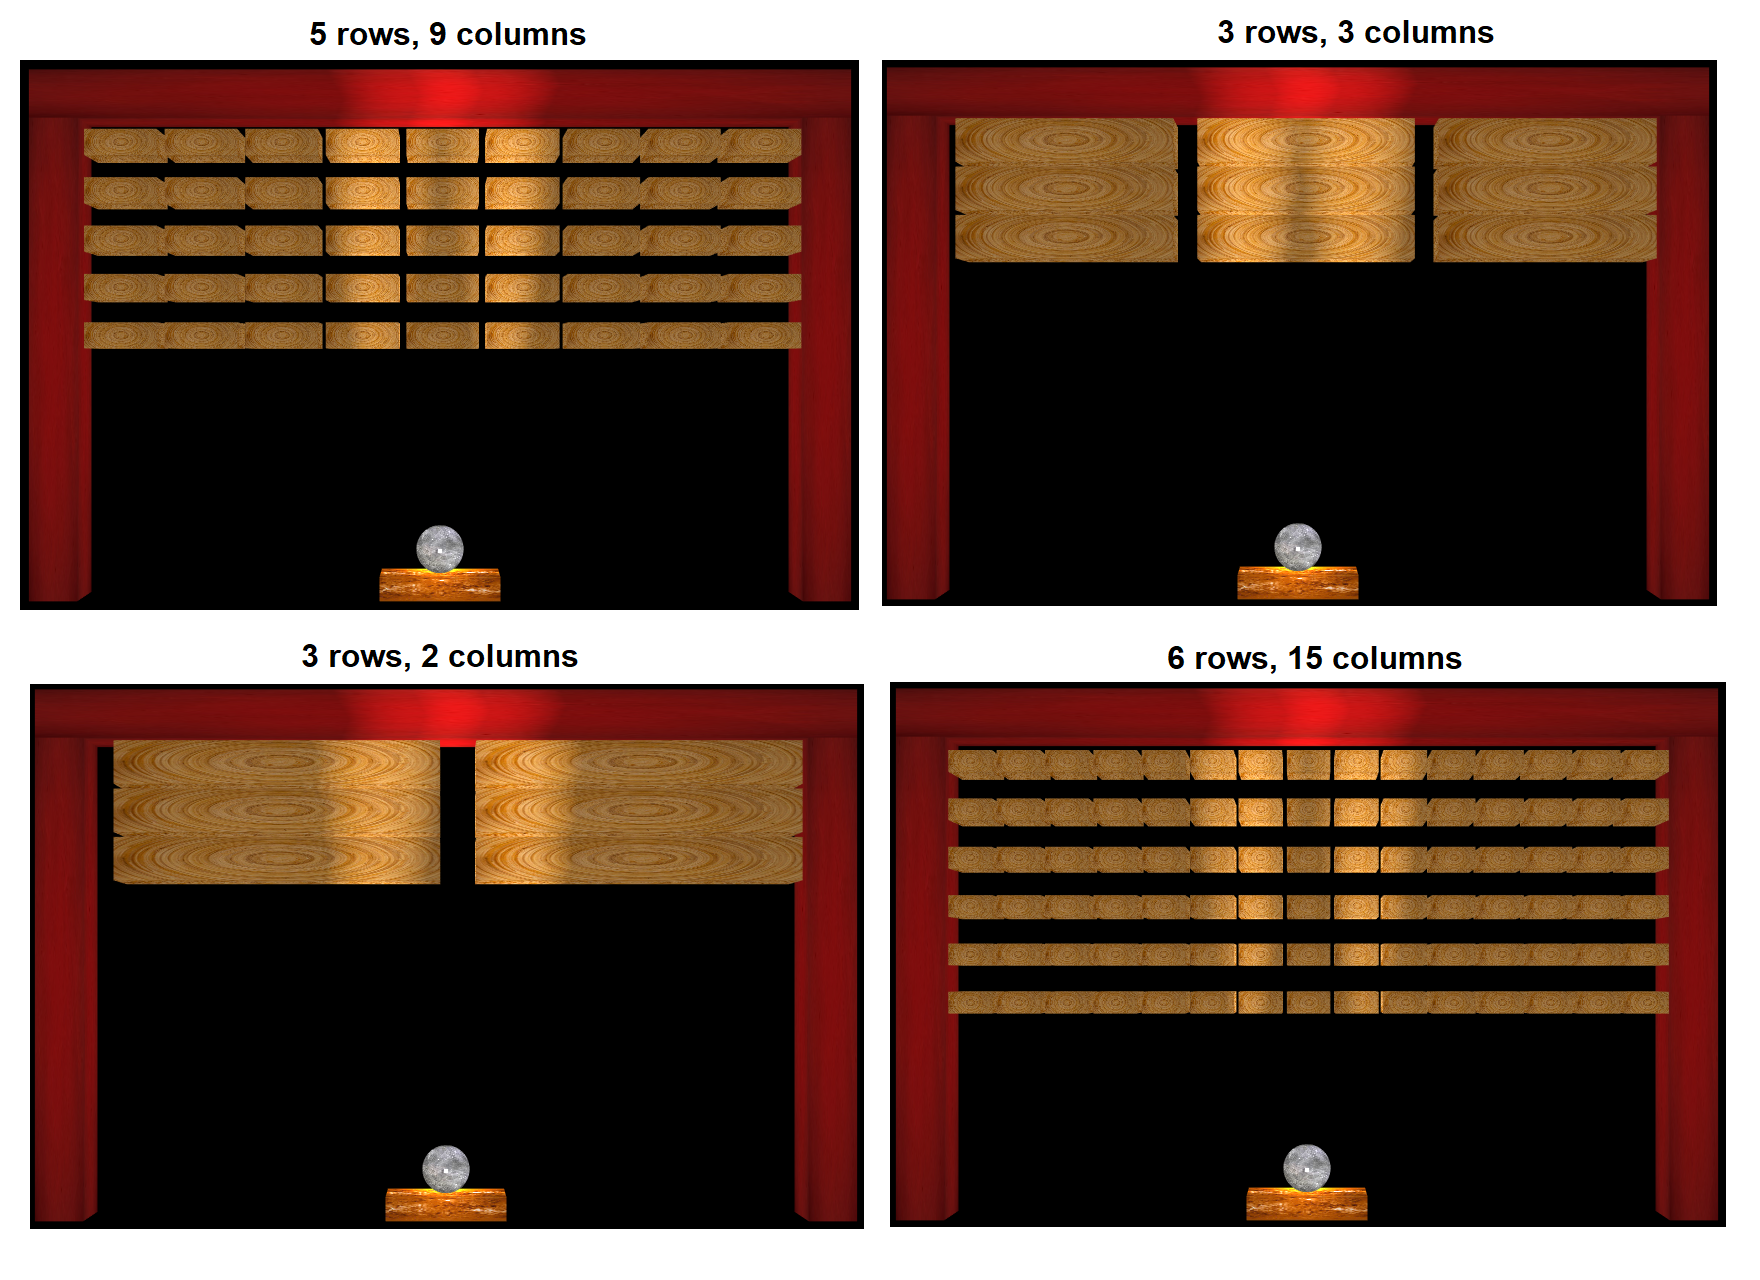
\includegraphics[width=\textwidth]{Images/SceneStart.png}
	\caption{Image at the start of the scene with different number of bricks. Number of rows and columns can be defined from \textbf{game.js}}
\end{figure}

The scene graph used was a simple one. Essentially it first goes trough all the lights, so that each object is affected by each light source, then everything else is initialised. The movements are instead handled by the physics system.
\begin{figure}[H]
	\centering
	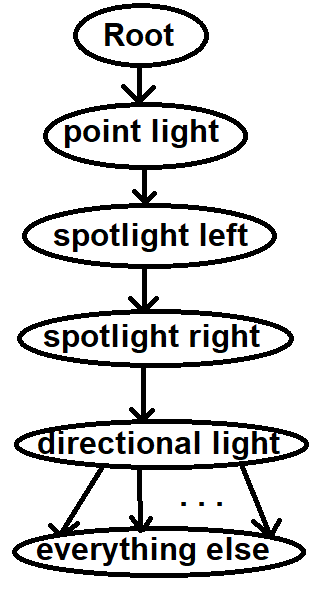
\includegraphics[width=0.3\textwidth]{Images/SceneGraph.png}
	\caption{Graphical representation of the scene graph}
\end{figure}

The appropriate materials are applied to the objects, with the proper materials to make them diffuse and specular as necessary. The walls, bricks and platform are diffuse, while the balls, powerups and bullets have a specular material.
\pagebreak
\chapter{Camera}
The camera in this game has a perspective view and always looks at the origin. The camera can be moved by using the W and S keys. The speed with which the camera can move may be altered using the T(slower) and R(faster) keys. Pressing Q puts the camera at the maximum angle and pressing E restores the camera view to normal (ie facing forwards). The parameters for this are found within \textbf{game.js} while the logic is found in the \textit{animate} function within \textbf{script.js}.

\begin{figure}[H]
	\centering
	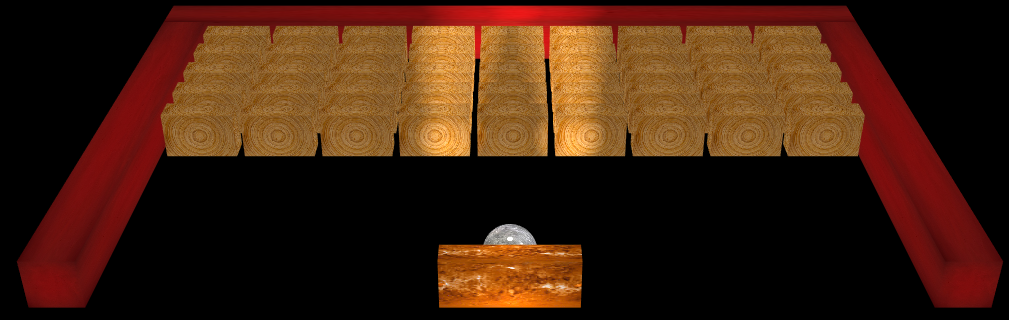
\includegraphics[width=\textwidth]{Images/Grazing.png}
	\caption{Camera looking a the scene at a grazing angle}
\end{figure}
\pagebreak
\chapter{Physics}
A custom physics engine was created for the game. The \textbf{physics.js} file contains the physics needs for the game.

First of all, physics objects are created. Two were defined for this game:
\begin{itemize}
	\item \textit{RectObject}, which has a width and height
	\item \textit{CircObject}, which hs a radius
\end{itemize}
Both of these 2 objects have a position (array of size 2, representing the x and y coordinates on the screen) and a velocity (array of size 2, representing the x and y velocity).

Some function which were defined and used were the following:
\begin{itemize}
	\item \textit{euclidean\un distance}: Given 2 points, it gets the euclidean distance between them
	\item \textit{CollisionRectCirc}: Takes a rectangle and a circle and returns if they intersect or not. Note: This does not consider the possibility of the circle being completely inside the square or vice versa. This function returns a collision type, whether the circle intersects with the top, bottom, left, bottom left, top right, etc, of the rectangle. Use fro collision between balls or bullets or powerups with the walls, bricks platform or other balls, as appropriate (for example: platform with brick collision does not make sense to check for).
	\item \textit{CollisionCircCirc}: Given 2 circles, checks if the 2 circles intersect by computing the distance between them and checks that this is smaller than te sum of their 2 radii.
	\item \textit{getDirectionVector}: Given 2 points, this returns a normalised direction vector from one position to the other. Used for when 2 balls collide with each other.
	\item \textit{multiply}: Multiplies a 2D vector by a scalar
	\item \textit{changeVelocityFromPoint}: While retaining the magnitude of the velocity vector given, it redirects such that it is now moving away from a specific point. This is used for when the ball collides with th platform. A point under the platform is used to shoot the ball away from the platform. Visually:
	\begin{figure}[H]
		\centering
		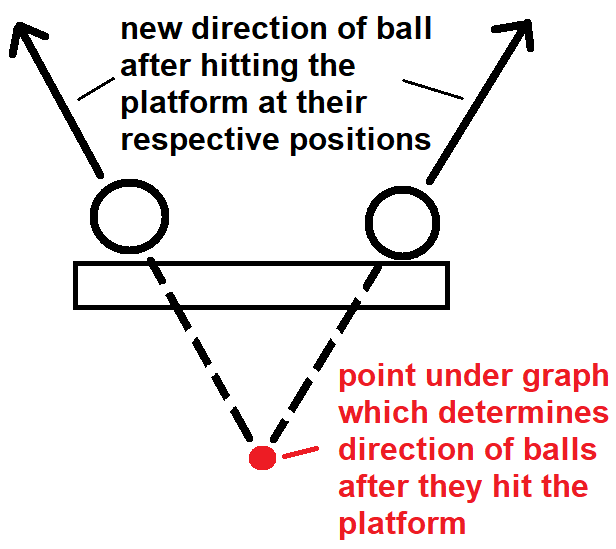
\includegraphics[width=0.3\textwidth]{Images/BallPlatform.png}
		\caption{Explanation of how ball rebounds off of platform}
	\end{figure}
	\item \textit{move}: Increments position of an object by its velocity
	\item \textit{moveMultiply}: Increments position of an object by its velocity vector multiplied by some amount
\end{itemize}

The physics engine is used within the animate function in \textbf{script.js}. The physics objects are initialised at the start for each object needed. Then within the animate function, the platform first moves, by checking user input of the right and let arrows. Then the ball and any other item which has a velocity is moved using the \textit{move} function. Afterwards, the collisions are computed and actions are taken accordingly. If a brick is hit, this is removed from the scene graph and the ball's velocity is rebounded accordingly. If a wall is hit the ball also rebounds. Then the actual nodes in the scene graph are moved according to the position of their respective physics objects.

When the game starts the ball is positioned in the middle of the platform, which can move left to right with the ball. Pressing spacebar releases the ball. Holding spacebar increases the launch velocity of the ball. If the ball falls down the pit, then it is reset on top of the spacebar. At 3 deaths, or when the player destroys all the bricks, the game is reset.
\pagebreak
\chapter{Additional Illumination}
\pagebreak
\chapter{Powerups}

The 6 powerups and their implementation will be discussed separately. Most powerups' duration was handled by having 2 variables: The duration of the powerup and the time when the powerup was collected. Then the program would know that a powerup is active or not if:
\[ Now < Duration + StartTime \]
As such, the StartTime would need to be initialised to \textit{Now - Duration}, otherwise all powerups would be active at the start of the game. When a powerup is collected, the StartTime for that powerup would be set to \textit{Now}. Other powerups which do not work with time (such as the bullets, where the player has a limited amount of them) are explicitly stated how they work in their respective section.

The powerup objects were implemented by having an object pool of 10 powerups and these would be spawned at position \textit{[100, 100]} with 0 velocity. Then when a brick is hit, the powerup has a 50\% of appearing and the powerup physics object would be placed upon the brick with velocity \textit{[0, SomeDownwardsVelocity]}. The actual rendered object is placed on the physics object automatically(since this is done each frame). When the powerup ball hits the platform, a random powerup is given to the player with equal probability. The powerup would then be put away from the screen and its velocity reset.

\begin{figure}[H]
	\centering
	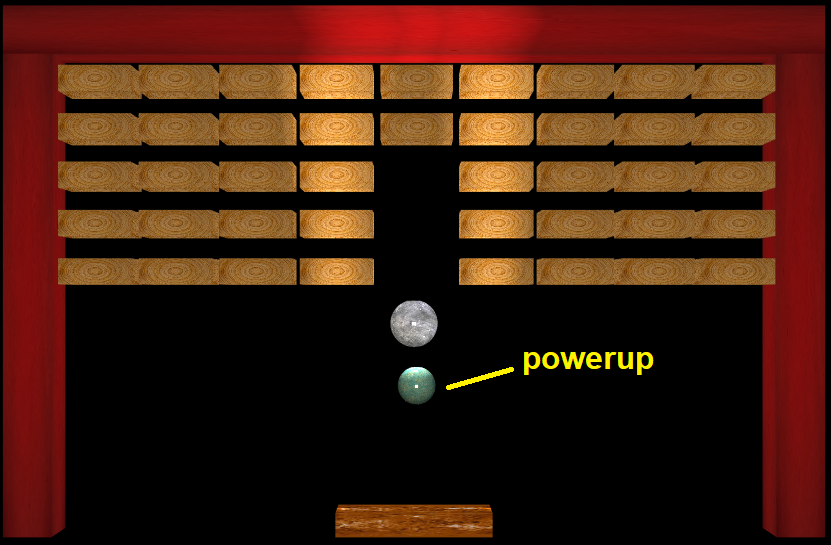
\includegraphics[width=0.7\textwidth]{Images/powerup.png}
	\caption{Image showing the powerup. Notice the light on top caused by the ball's point light}
\end{figure}

\section{Moving trough bricks}
For this powerup, it was a matter of simply making a condition where if the powerup is active (using the time method stated above) the ball's velocity would remain constant when hitting a brick. Then it would be rebounded once it hits the wall or platform. Note: this powerup only works on the main ball, not the additional balls as well. This powerup may be seen in the video at 00:24.

\section{Resizing the platform}
For this, the platform width is changed. This is done by having an \textit{initialWidth} variable as well as a \textit{multiplier} variable which was set to 1.3 (ie the platform will be 1.3x of it's initial size). Then at each frame, the width is changed according to whether the powerup is active or not, and everything regarding the platform depends on this width so it all changes accordingly (such as the point lights' positions).  This powerup may be seen in the video at 00:23.

\section{Additional Balls}
A pool of additional balls was created and, just like the powerups themselves, these were placed away from the screen and set with velocity 0. When the additional ball powerup is collected, this spawns a new ball next to the main ball with the same velocity. The position of the new ball is determined based on the position of the ball with regards to screen space. If the ball is on the left side of the screen, then the additional ball is spawned on the ball's right and vice versa. Important to note is that any powerup which the main balls have, these are not shared by the additional balls. This was to make the additional balls act like basic balls, while the main ball is special. The main ball and additional balls can collide with each other, and when they do, they get reflected so that they go in opposite directions of each other. A check is made in the animate loop so that if the ball starts moving just horizontally (ie gets stuck bouncing between the horizontal walls) it gets a bit of a velocity downwards. This powerup may be seen in the video at 00:30.

\begin{figure}[H]
	\centering
	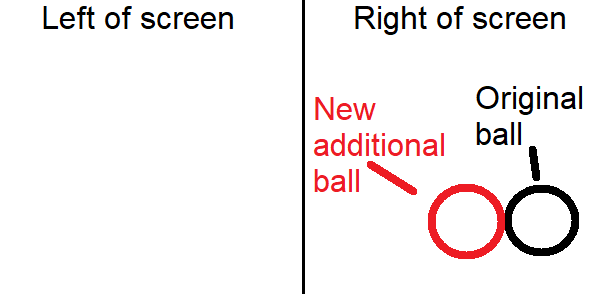
\includegraphics[width=0.7\textwidth]{Images/AdditionalBall.png}
	\caption{Image showing how additional balls are spawned. Since the ball is on the right side of the screen, the new additional ball is spawned on the left of the main ball}
\end{figure}

\section{Slow Ball}
When moving the ball in the animate loop, a check is made to see if the slow moving powerup is active. If it is, the ball moves at half speed using the \textit{moveMultiply} method discussed in the physics section. Note: This powerup only acts on the main ball and not the additional ones as well. This powerup may be seen in the video at 00:06.

\section{Sticky Platform}
For this powerup, the ball can stick the the platform 2 times after picking up the powerup. A check is made when the main ball hits the platform to see if the ball can still stick to the platform. If the amount is more than 0 then the ball sticks, meaning that the ball's velocity goes to zero and the scenario goes back like the beginning of the game, with the ball being able to be launched using spacebar. The ball can still reflect off additional balls while in this form. The \textit{ballIsStuck} boolean is used to check if the ball is stuck to the platform.  This powerup may be seen in the video at 00:26.

\section{Cannon}
For this, an amount of bullets is given to the player. At the start this number is 0. When the player gets this powerup, this number goes to 3, so that the player has 3 bullets to shoot. If the player has some remaining bullets from the previous powerup he got, then the player goes back up to 3, ie the number of bullets is capped at 3. The player can then shoot these bullets if he presses the UP-ARROW. Note: An object pool is used for the bullets. This powerup may be seen in the video at 00:46.

\begin{figure}[H]
	\centering
	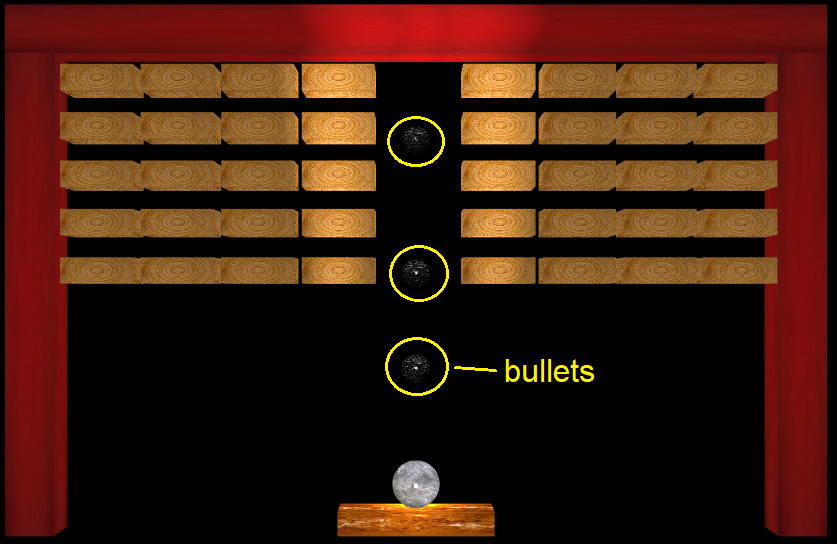
\includegraphics[width=0.7\textwidth]{Images/bullets.png}
	\caption{Image showing the bullets in the game}
\end{figure}
\pagebreak
\chapter{Extras}
To make the game more enjoyable, it was decided to add some additional features, which while they do not change the mechanics of the game, they make the game look nicer and feel more rewarding.

\section{Music}
The first of these is the music and sound effects. These were implemented by referencing within the HTML file then playing them trough javascript when the event when they should play happens. The music is a looped song which plays when the player first shoots the ball. Sound effects also play for the following events:
\begin{itemize}
	\item Destroying brick
	\item Shooting bullet
	\item Charging up the platform to shoot the ball (Also acts as an audio queue to show when max speed has been reached)
	\item Ball hits the ground
	\item Balls collide
	\item Collecting powerup
	\item Hitting platform
	\item Hitting wall
	\item Winning
	\item Losing
\end{itemize}
The music was found on youtube audio library and the rest of the sound effects were found on youtube or freesound.org.

\section{Particles}
Particles are used in most modern games. These subtle yet very visually appealing explosions make the game look more natural and rewarding. Hence I put particles when bricks break. Although normally billboards are used for particles, this simple particle system uses a pool of spheres and takes four of that pool and spawns them where the brick broke for a fraction of a second. They appear, move towards a random direction and fade away (using scaling) so that they appear to fade away into nothing. An image showing the particles is very difficult to obtain as a single frame of these looks weird, hence please look at the video and notice at the small balls which appear when the bricks break.

\section{Background}
For this, a skybox and a tiling image of a starry sky was used. The skybox was made by simply wrapping the play area with a cube.
\pagebreak

\chapter{Conclusion}
%This concludes the report for the CPS2000-Compilers Assignment. For further information view the attached README to get info on directory structure and how to use the compiler. The video showcase includes some examples which show the compiler's functionality and features in action. The appropriate code and test cases were shown. 

%Inside the folder containing this report are the project files as sub-folders, including the README, CMakeLists and sample InputFiles to test the compiler with.


\pagebreak

\pagebreak
\chapter*{Appendix}\addcontentsline{toc}{section}{Appendix}

\section*{Plagiarism Form}
\begin{figure}[H]
	\centering
	\includegraphics[width=0.7\textwidth]{Images/plagiarismform.png}
\end{figure}
\end{document}